\documentclass[11pt,a4paper]{article}
\usepackage[margin=1in]{geometry}
\usepackage{graphicx,booktabs,float,subcaption,amsmath,enumitem,hyperref,microtype}
\hypersetup{hidelinks}
\graphicspath{{../figures/}}
\setlength{\parskip}{0.5em}\setlength{\parindent}{0pt}
\title{EN3150 Assignment 03\\Section 6: Final Comparison and Trade-off Discussion}
\author{Group Draco -- \textit{Dealing with AI from the core}}
\date{October 2026}
\begin{document}
\maketitle
\begin{center}
GUNARATHNA K.T.M.B. (230203G) \quad JAYAWARDANA K.P.P. (230294H)\\
JITHMAL P.G.I. (230306B) \quad NIMADITH W.N.A.C. (230442L)
\end{center}

\section{Final Comparison and Trade-off Discussion}
The final comparison focuses on Model B, MobileNetV2, and ShuffleNetV2 1.0x. Model A is retained only as a baseline in the Pareto plots. All three final candidates use the same packaged DeFungi split. Test metrics are measured from saved experiments; parameter counts and checkpoint sizes are reproducible from the code/files; MACs are calculated under one common Conv2d+Linear convention for a $3\times64\times64$ input.

\begin{table}[H]\centering\small
\caption{Final model comparison.}
\begin{tabular}{lrrrrr}
\toprule
Model & Test Acc. & Macro F1 & Parameters & Size & MACs\\
\midrule
Model B & 70.43\% & 0.6927 & 37,957 & 0.176 MiB & 7.26 M\\
ShuffleNetV2 1.0x & 83.76\% & 0.8590 & 1,258,729 & 4.966 MiB & 11.75 M\\
MobileNetV2 & 86.31\% & 0.8805 & 2,230,277 & 8.740 MiB & 24.45 M\\
\bottomrule
\end{tabular}
\end{table}

\subsection{Accuracy}
\begin{figure}[H]\centering
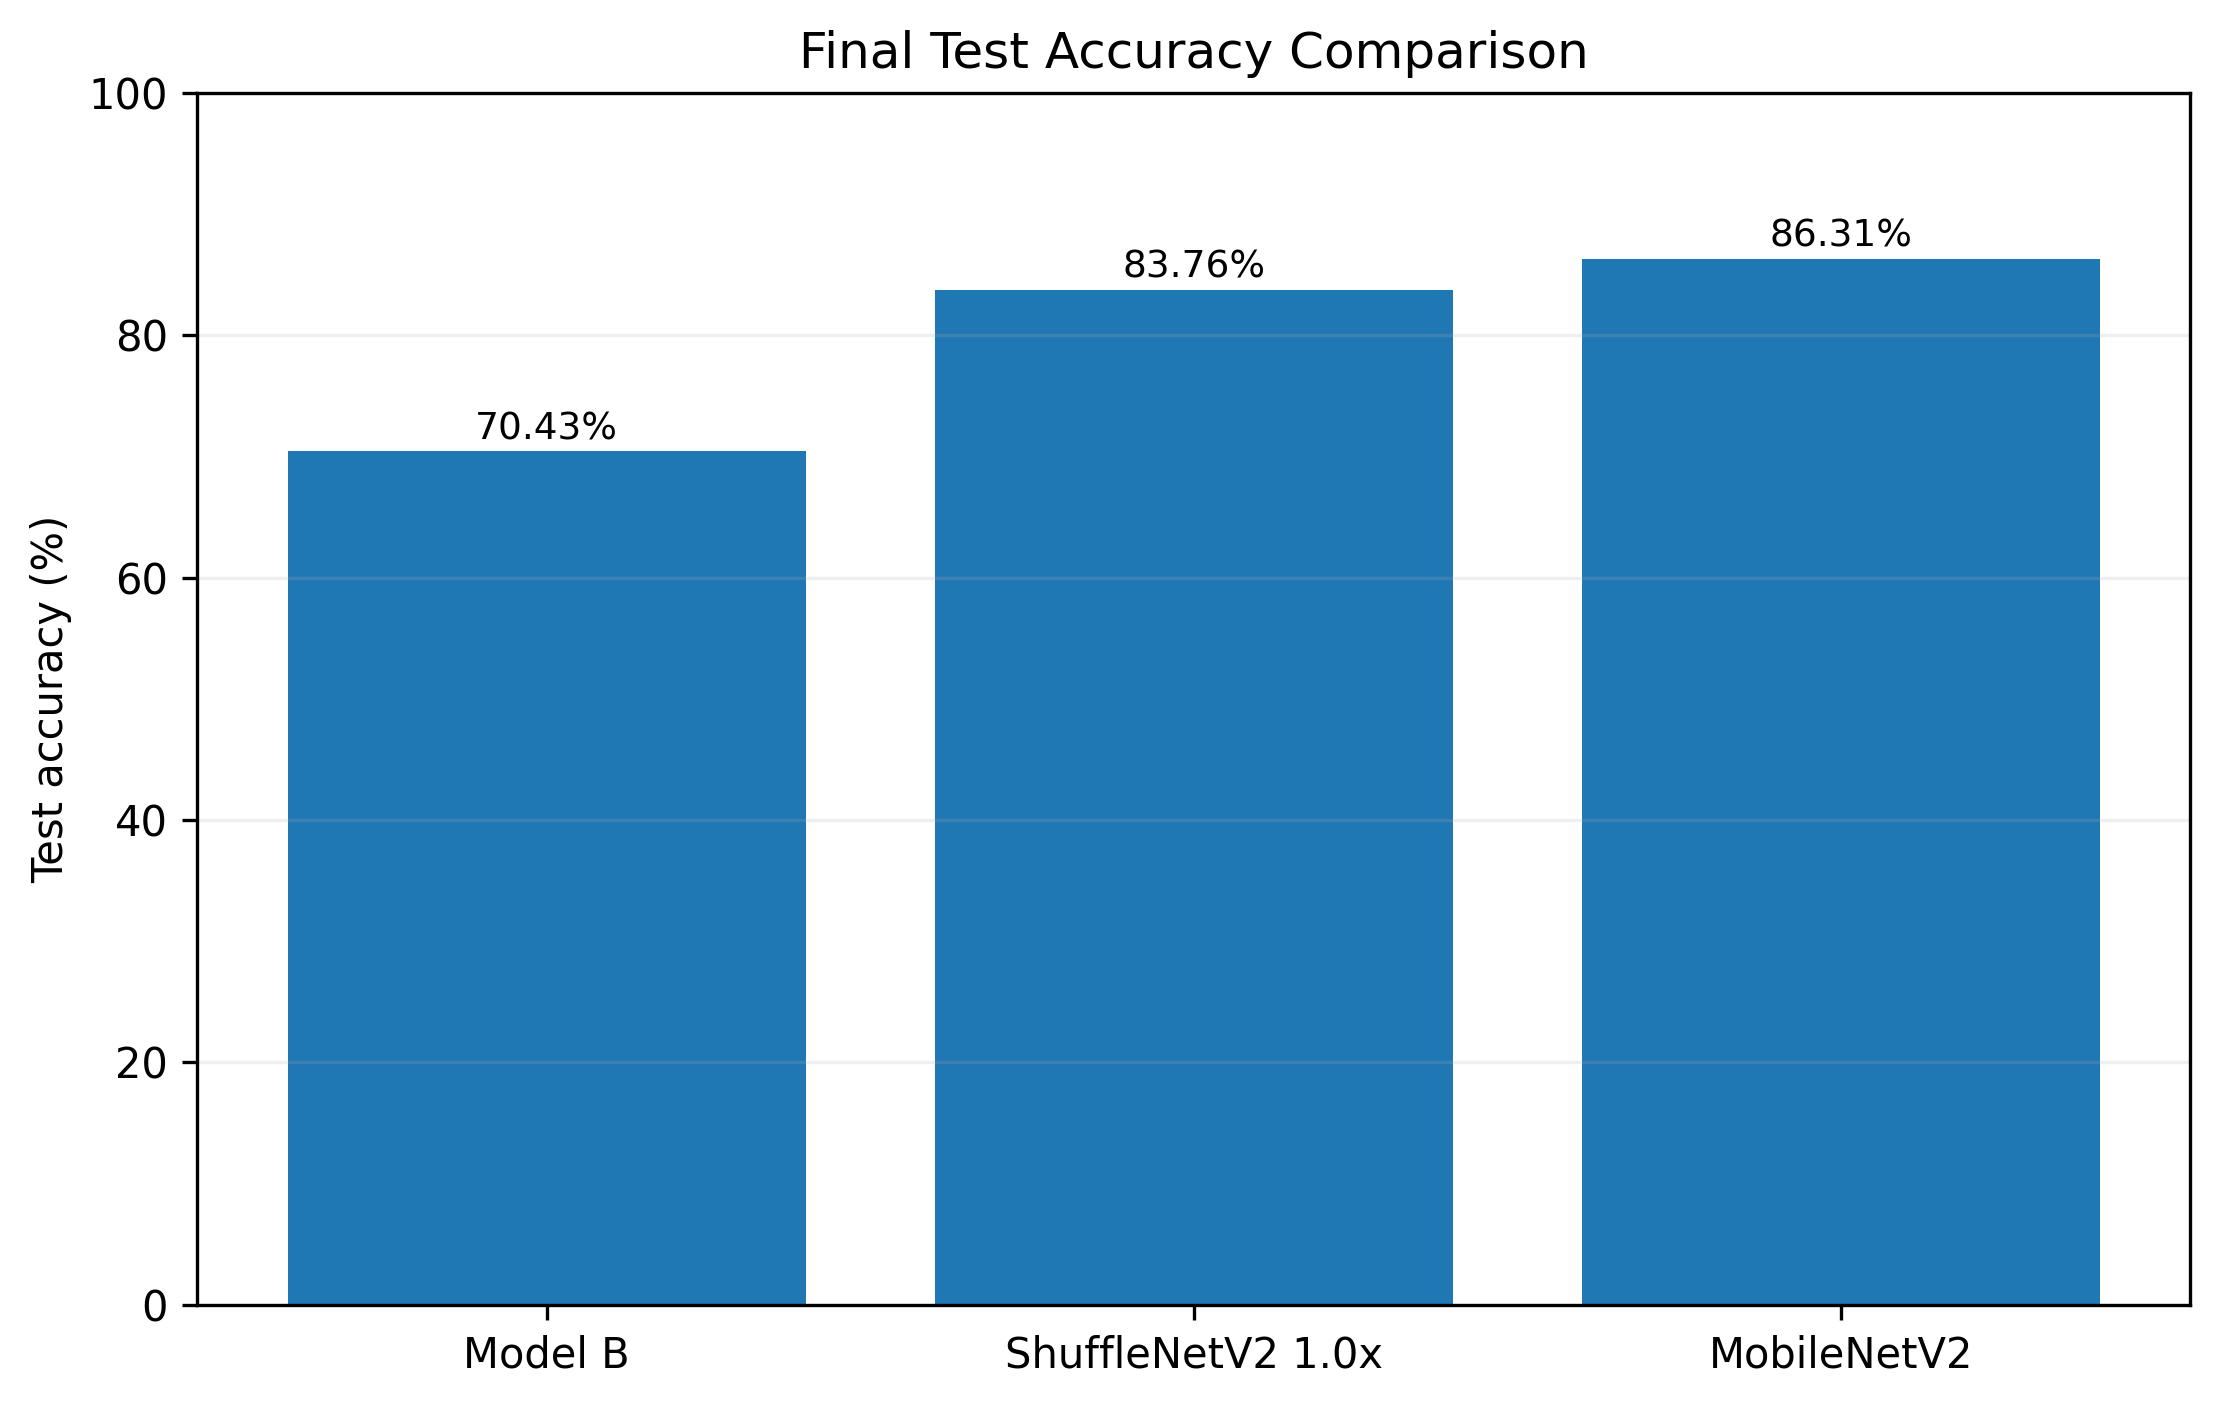
\includegraphics[width=.78\linewidth]{task6/test_accuracy_comparison.png}
\caption{Test accuracy.}
\end{figure}
MobileNetV2 improves on Model B by 15.88 percentage points, while ShuffleNetV2 improves by 13.33 percentage points. The pre-trained networks also improve class-wise robustness; H2 recall rises from 0.4387 for Model B to approximately 0.66 for ShuffleNetV2 and 0.77 for MobileNetV2.

\subsection{Memory Footprint}
\begin{figure}[H]\centering
\begin{subfigure}{.49\linewidth}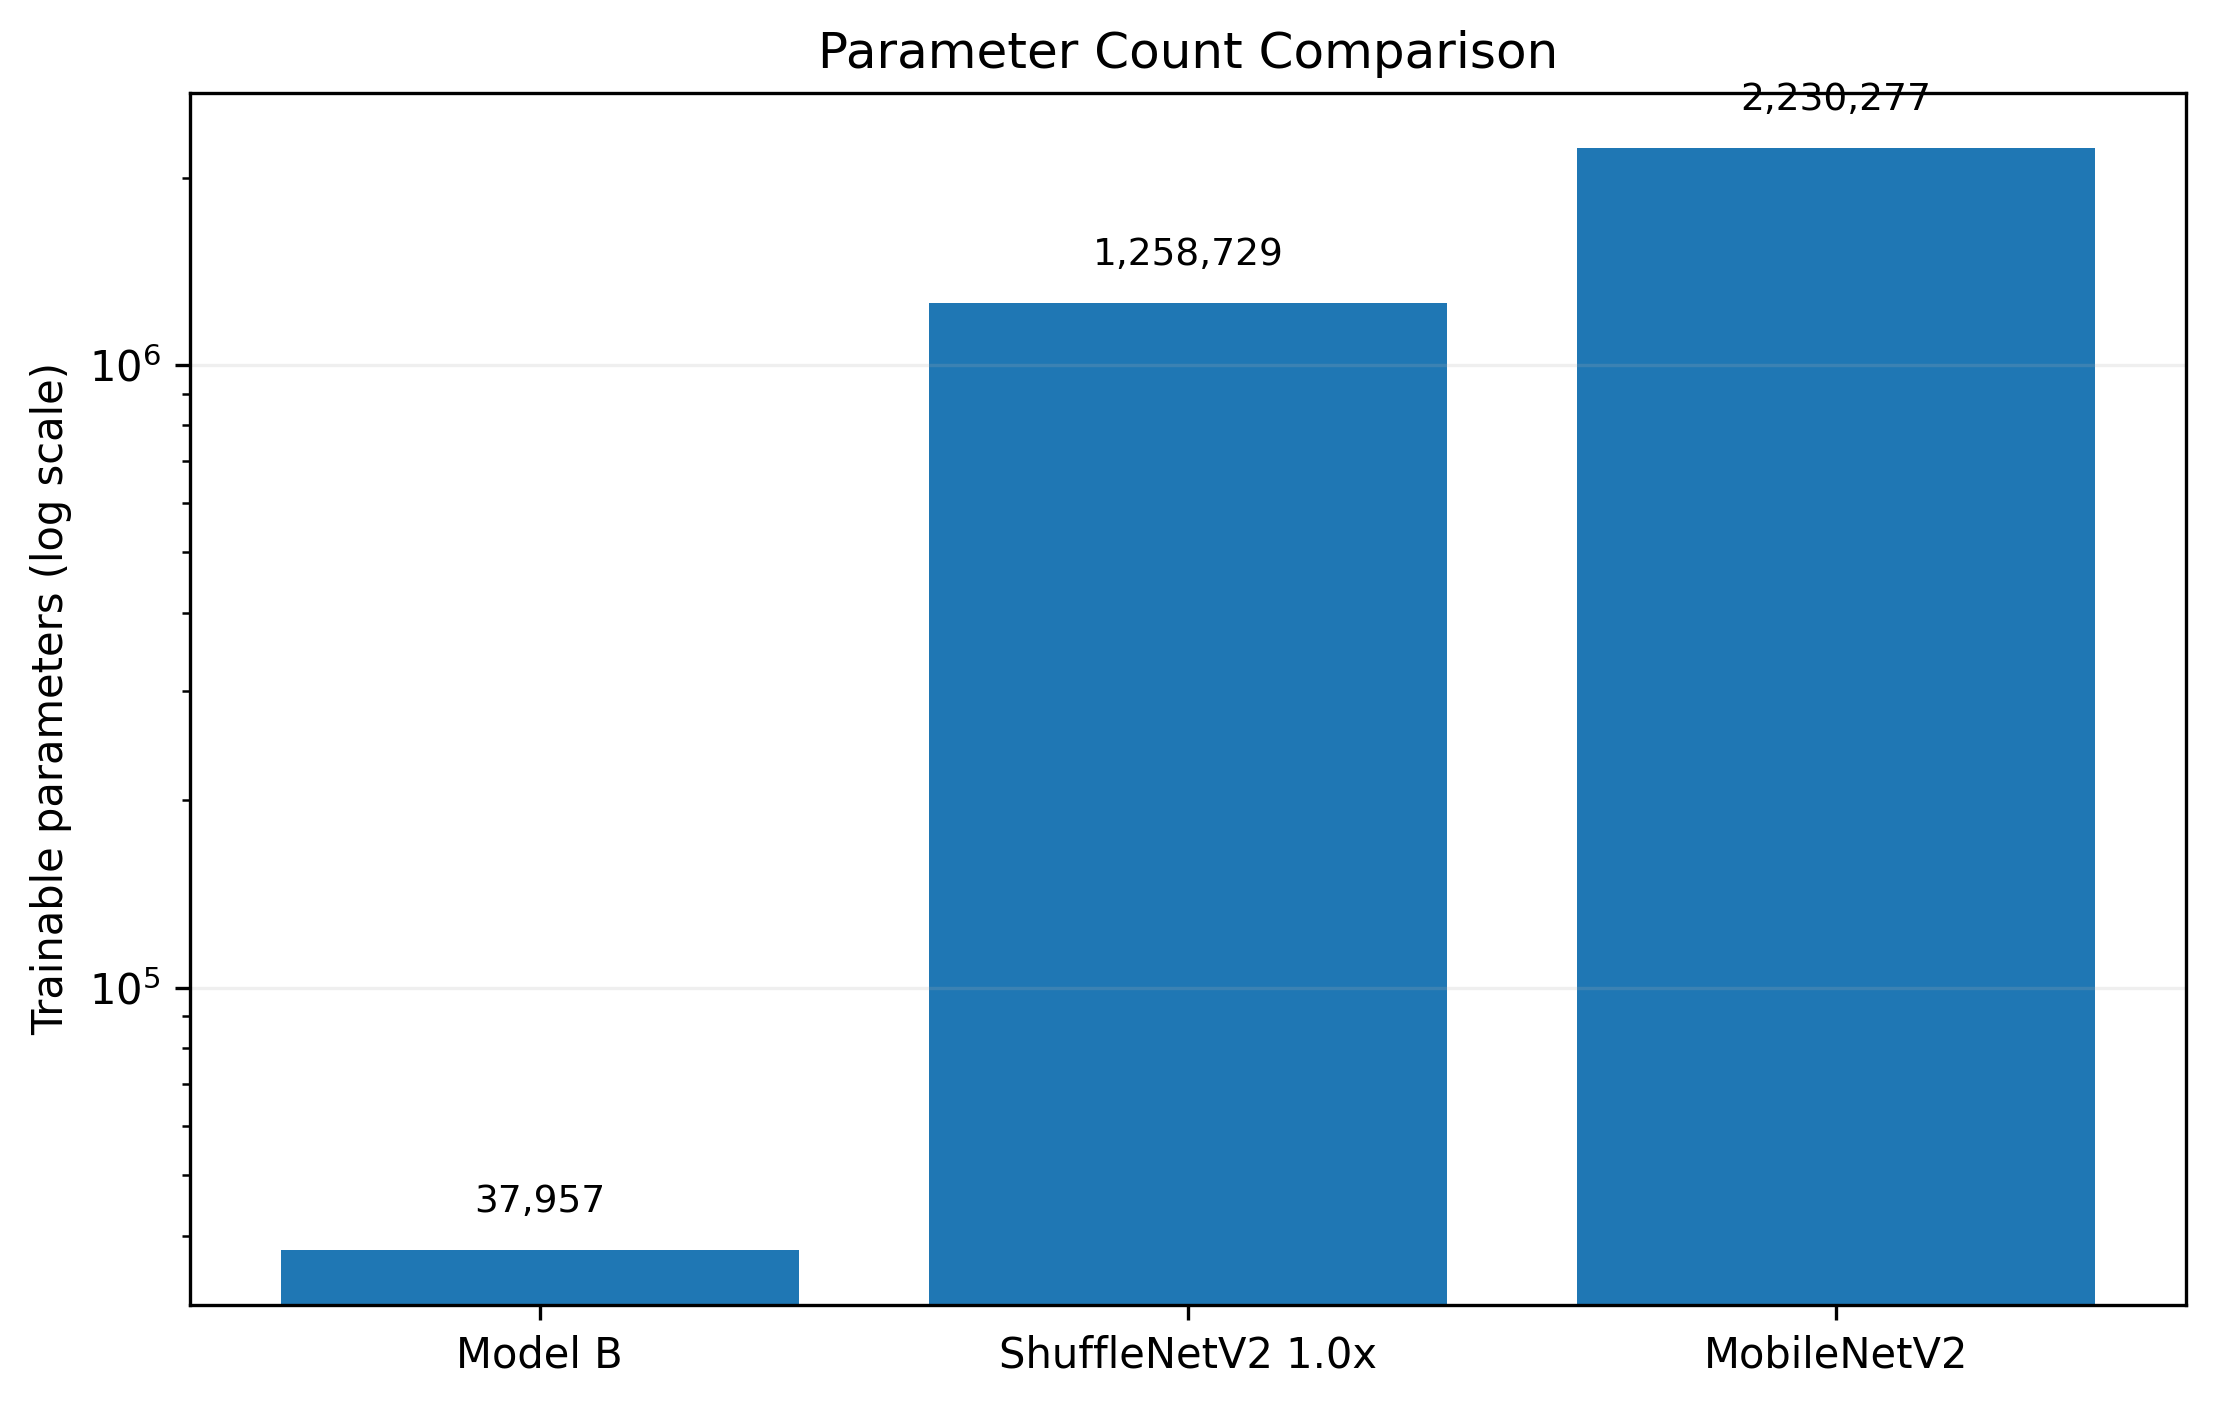
\includegraphics[width=\linewidth]{task6/parameter_count_comparison.png}\caption{Parameters.}\end{subfigure}\hfill
\begin{subfigure}{.49\linewidth}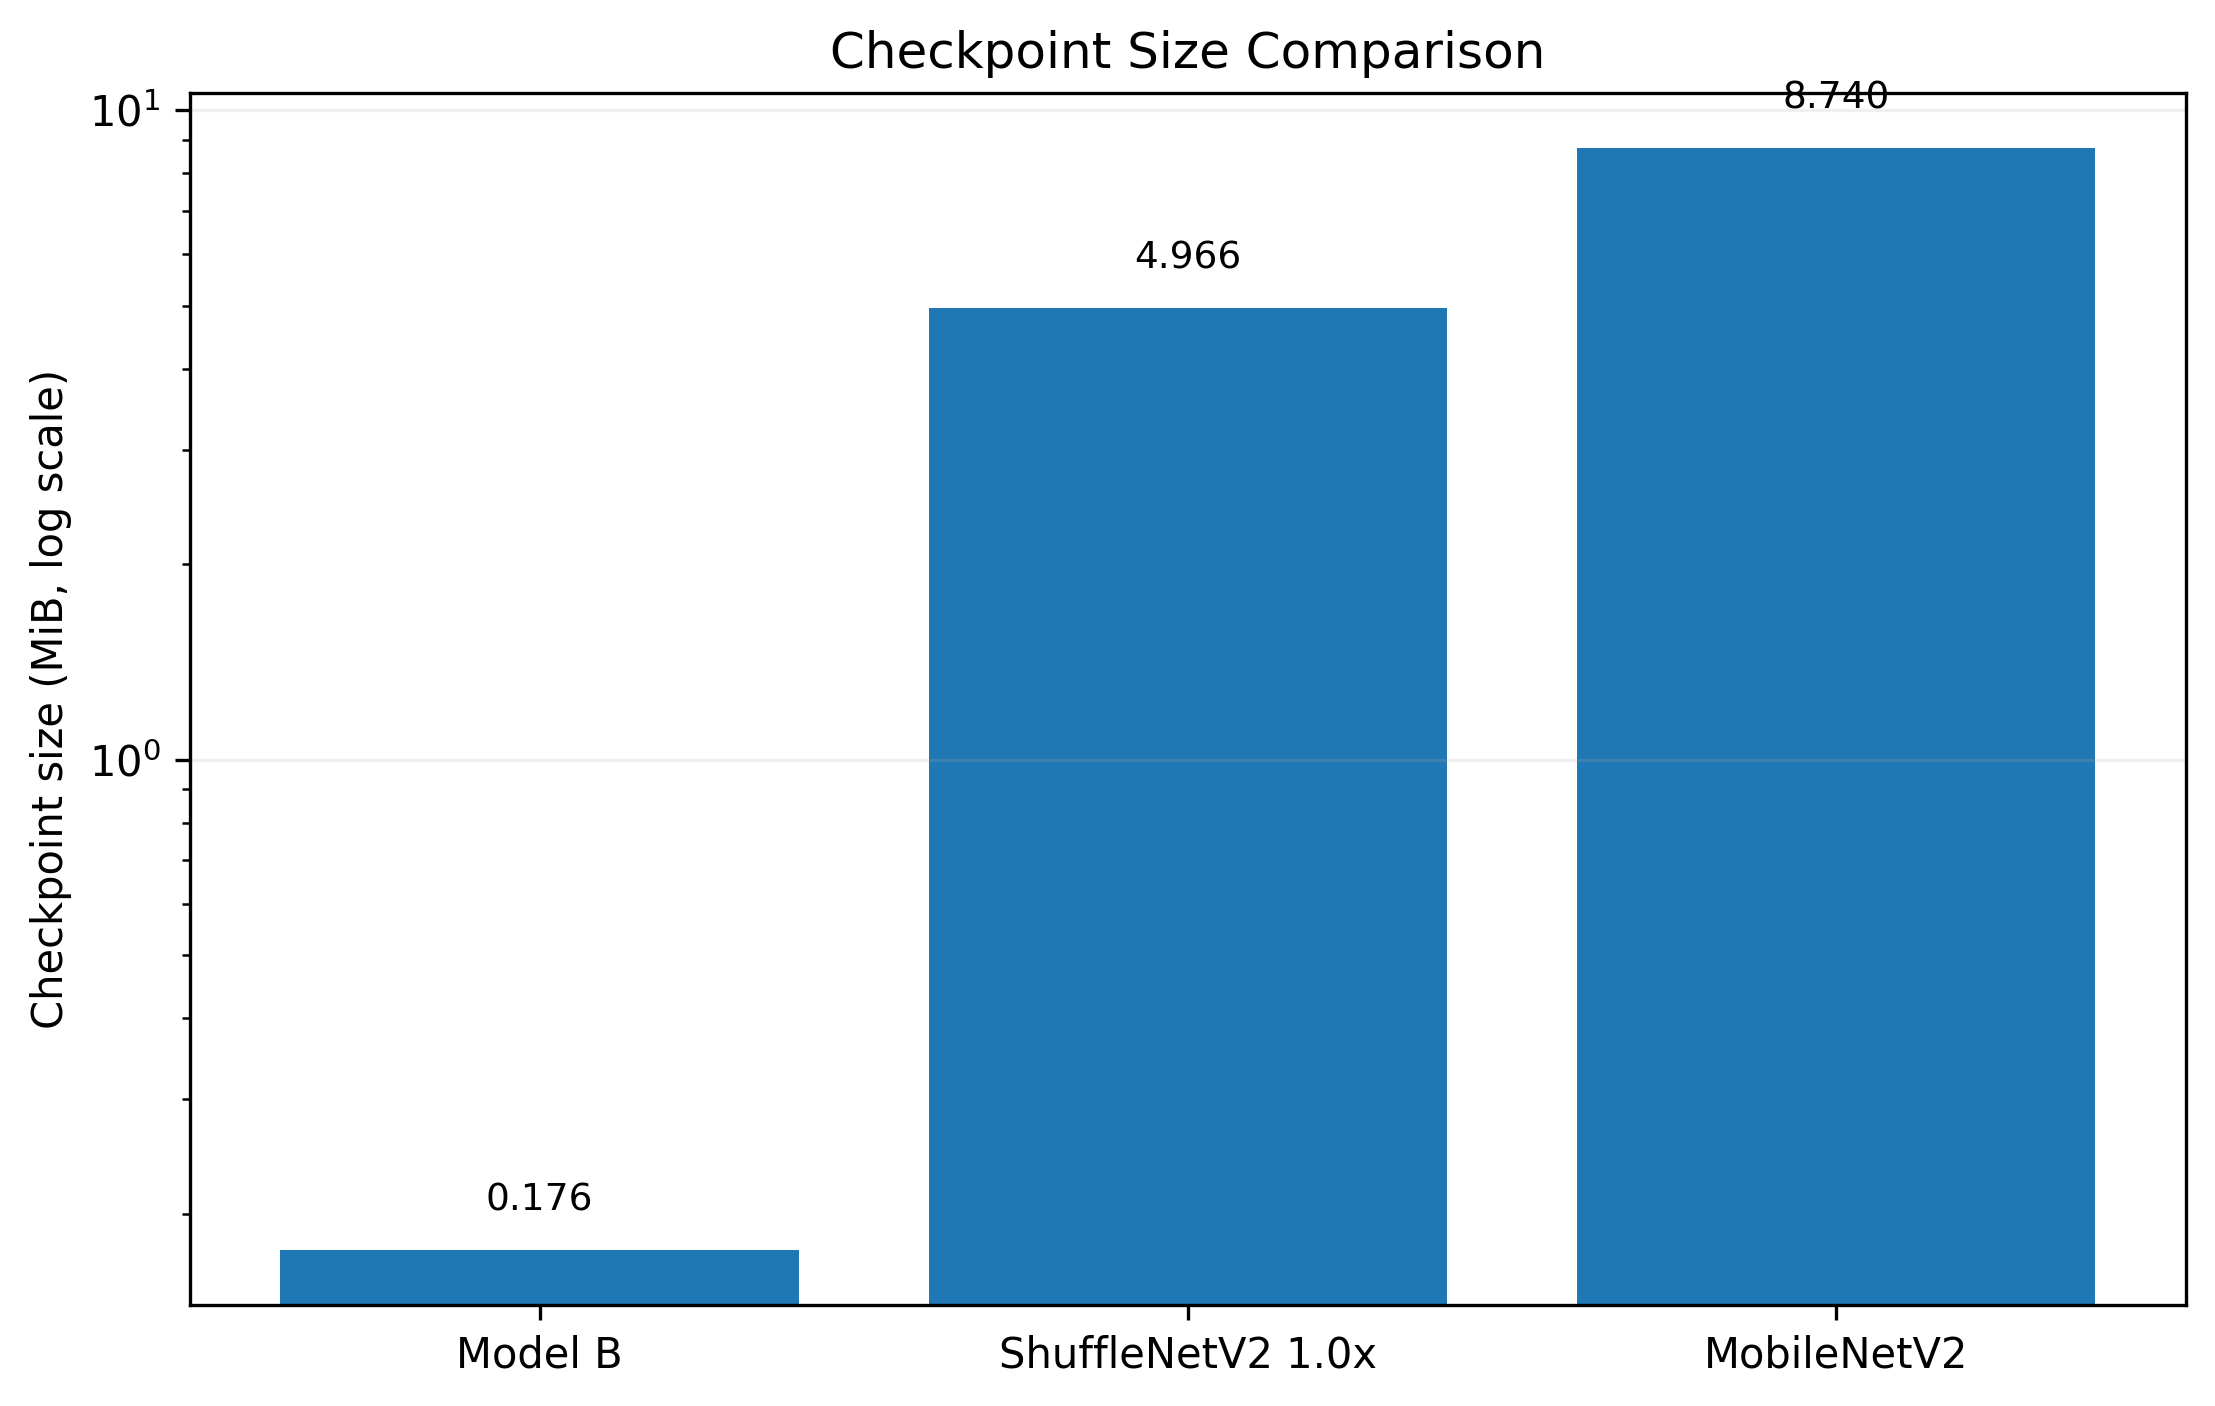
\includegraphics[width=\linewidth]{task6/model_size_comparison.png}\caption{Checkpoint size.}\end{subfigure}
\caption{Memory-related comparisons.}
\end{figure}
ShuffleNetV2 has 33.16$\times$ as many parameters and a 28.23$\times$ larger checkpoint than Model B. MobileNetV2 has 58.76$\times$ as many parameters and a 49.68$\times$ larger checkpoint. These file-size comparisons do not directly equal runtime RAM; peak activation buffers and framework/operator overhead must be measured on the target device.

\subsection{Computational Cost}
\begin{figure}[H]\centering
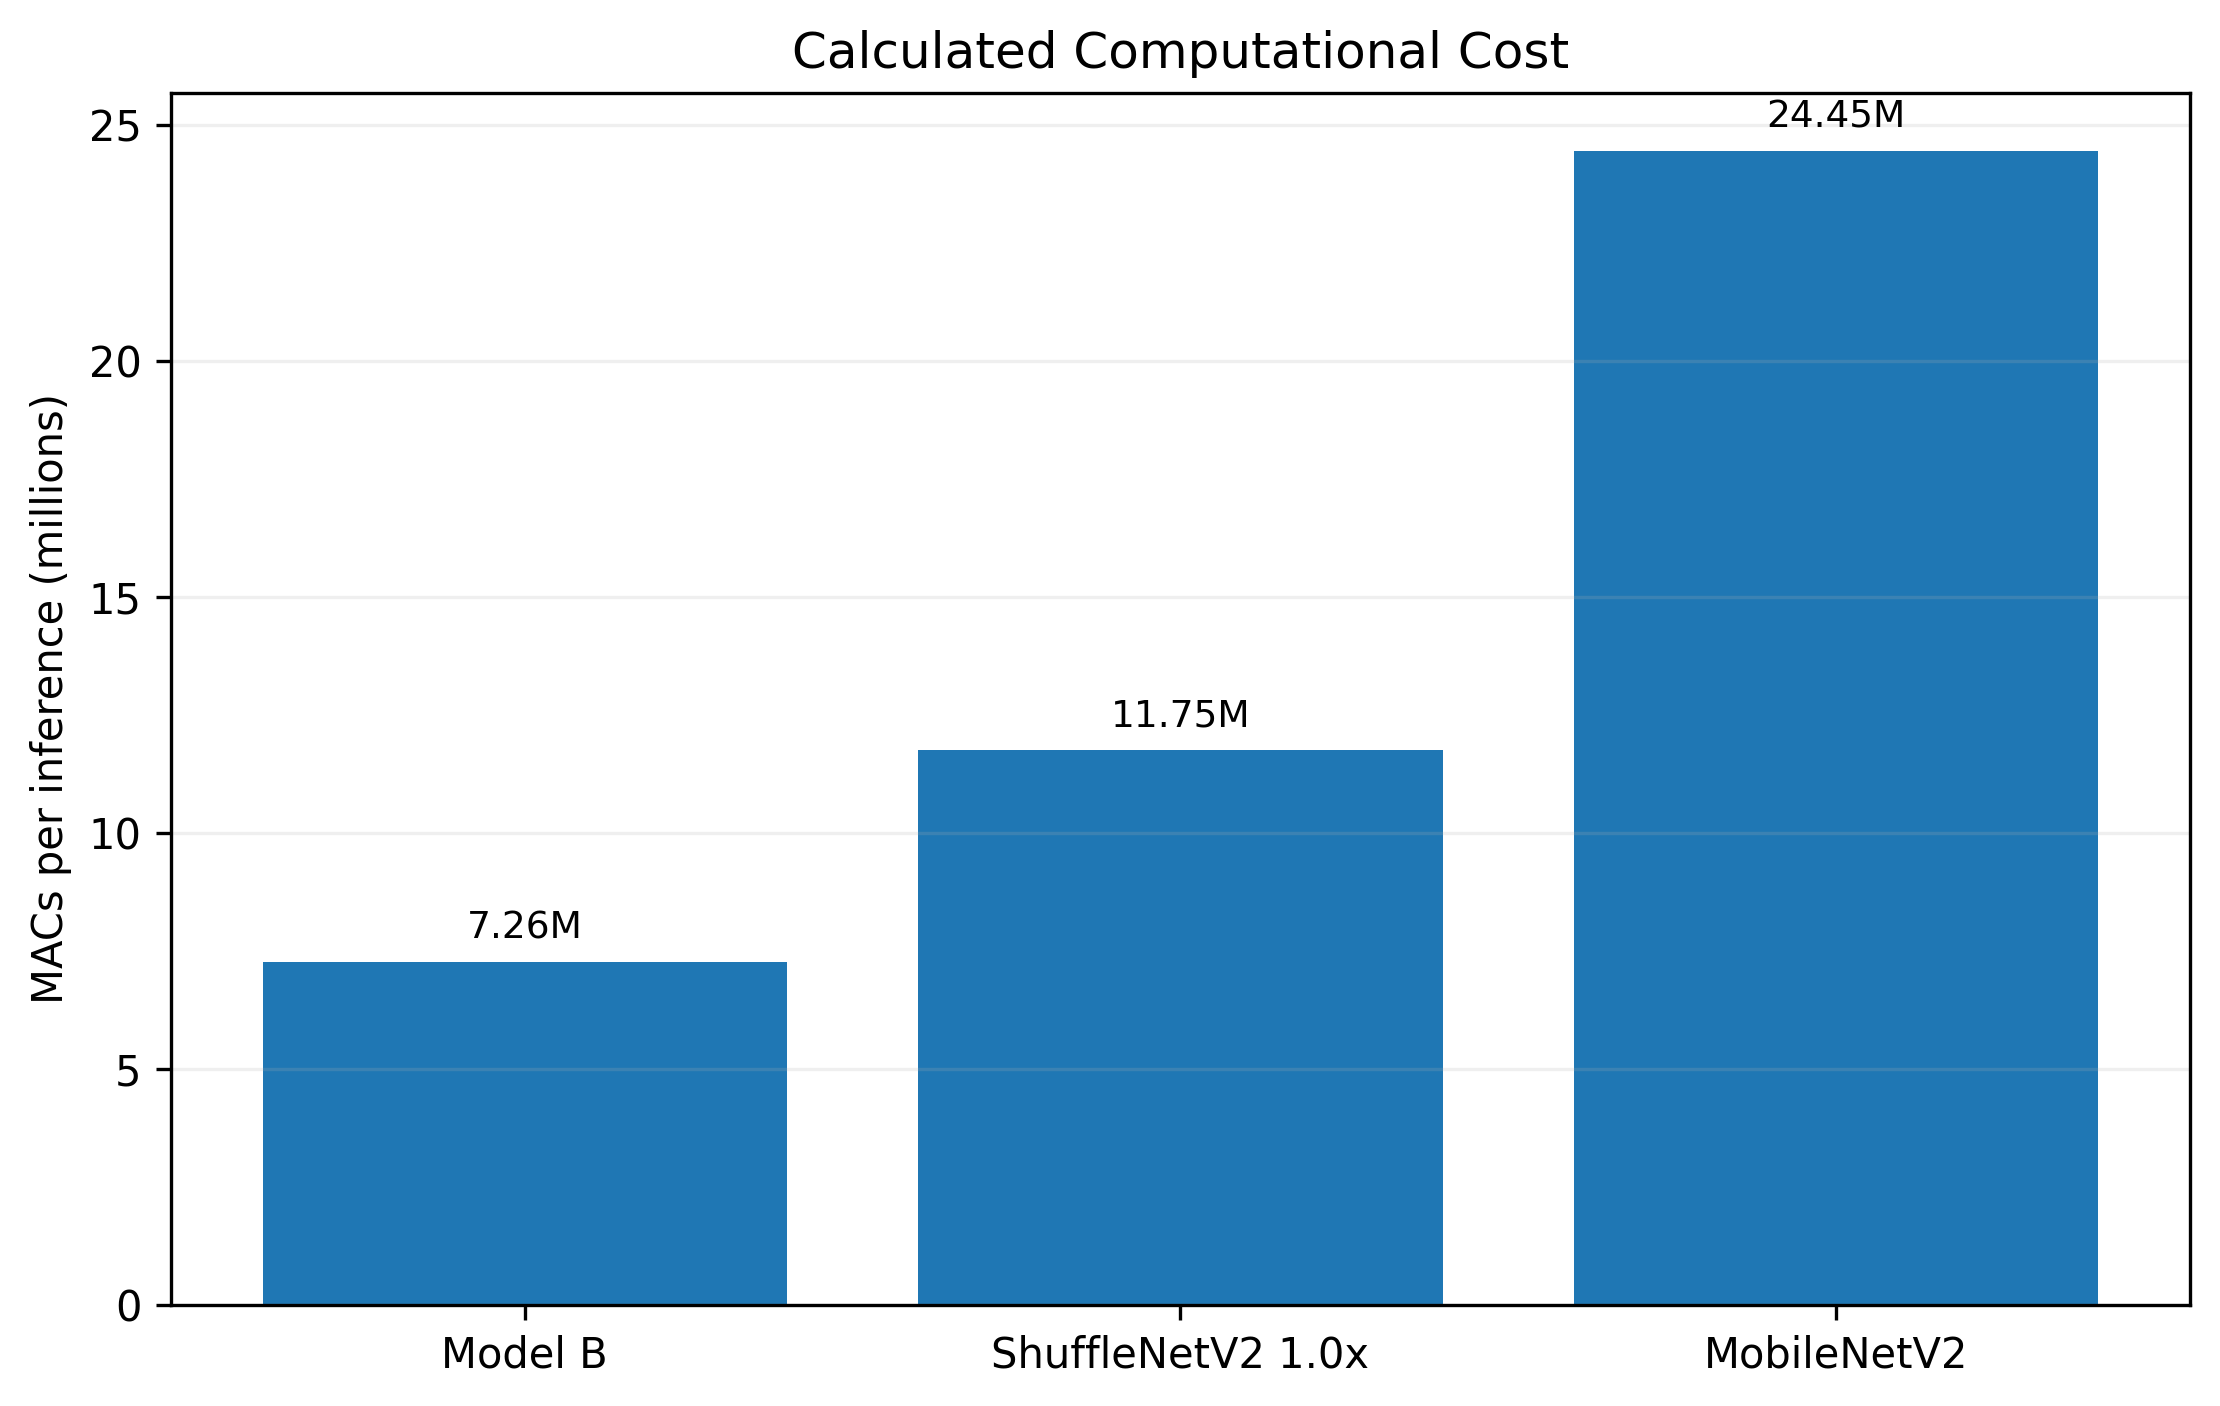
\includegraphics[width=.78\linewidth]{task6/mac_comparison.png}
\caption{Calculated Conv/Linear MACs per $64\times64$ image.}
\end{figure}
Model B requires 7.26 M MACs. ShuffleNetV2 requires 11.75 M (1.62$\times$ Model B), while MobileNetV2 requires 24.45 M (3.37$\times$ Model B). The project does not contain a valid controlled device-latency measurement, so no latency claim is made and training time is not used as a substitute.

\subsection{Accuracy-Efficiency Trade-offs}
\begin{figure}[H]\centering
\begin{subfigure}{.49\linewidth}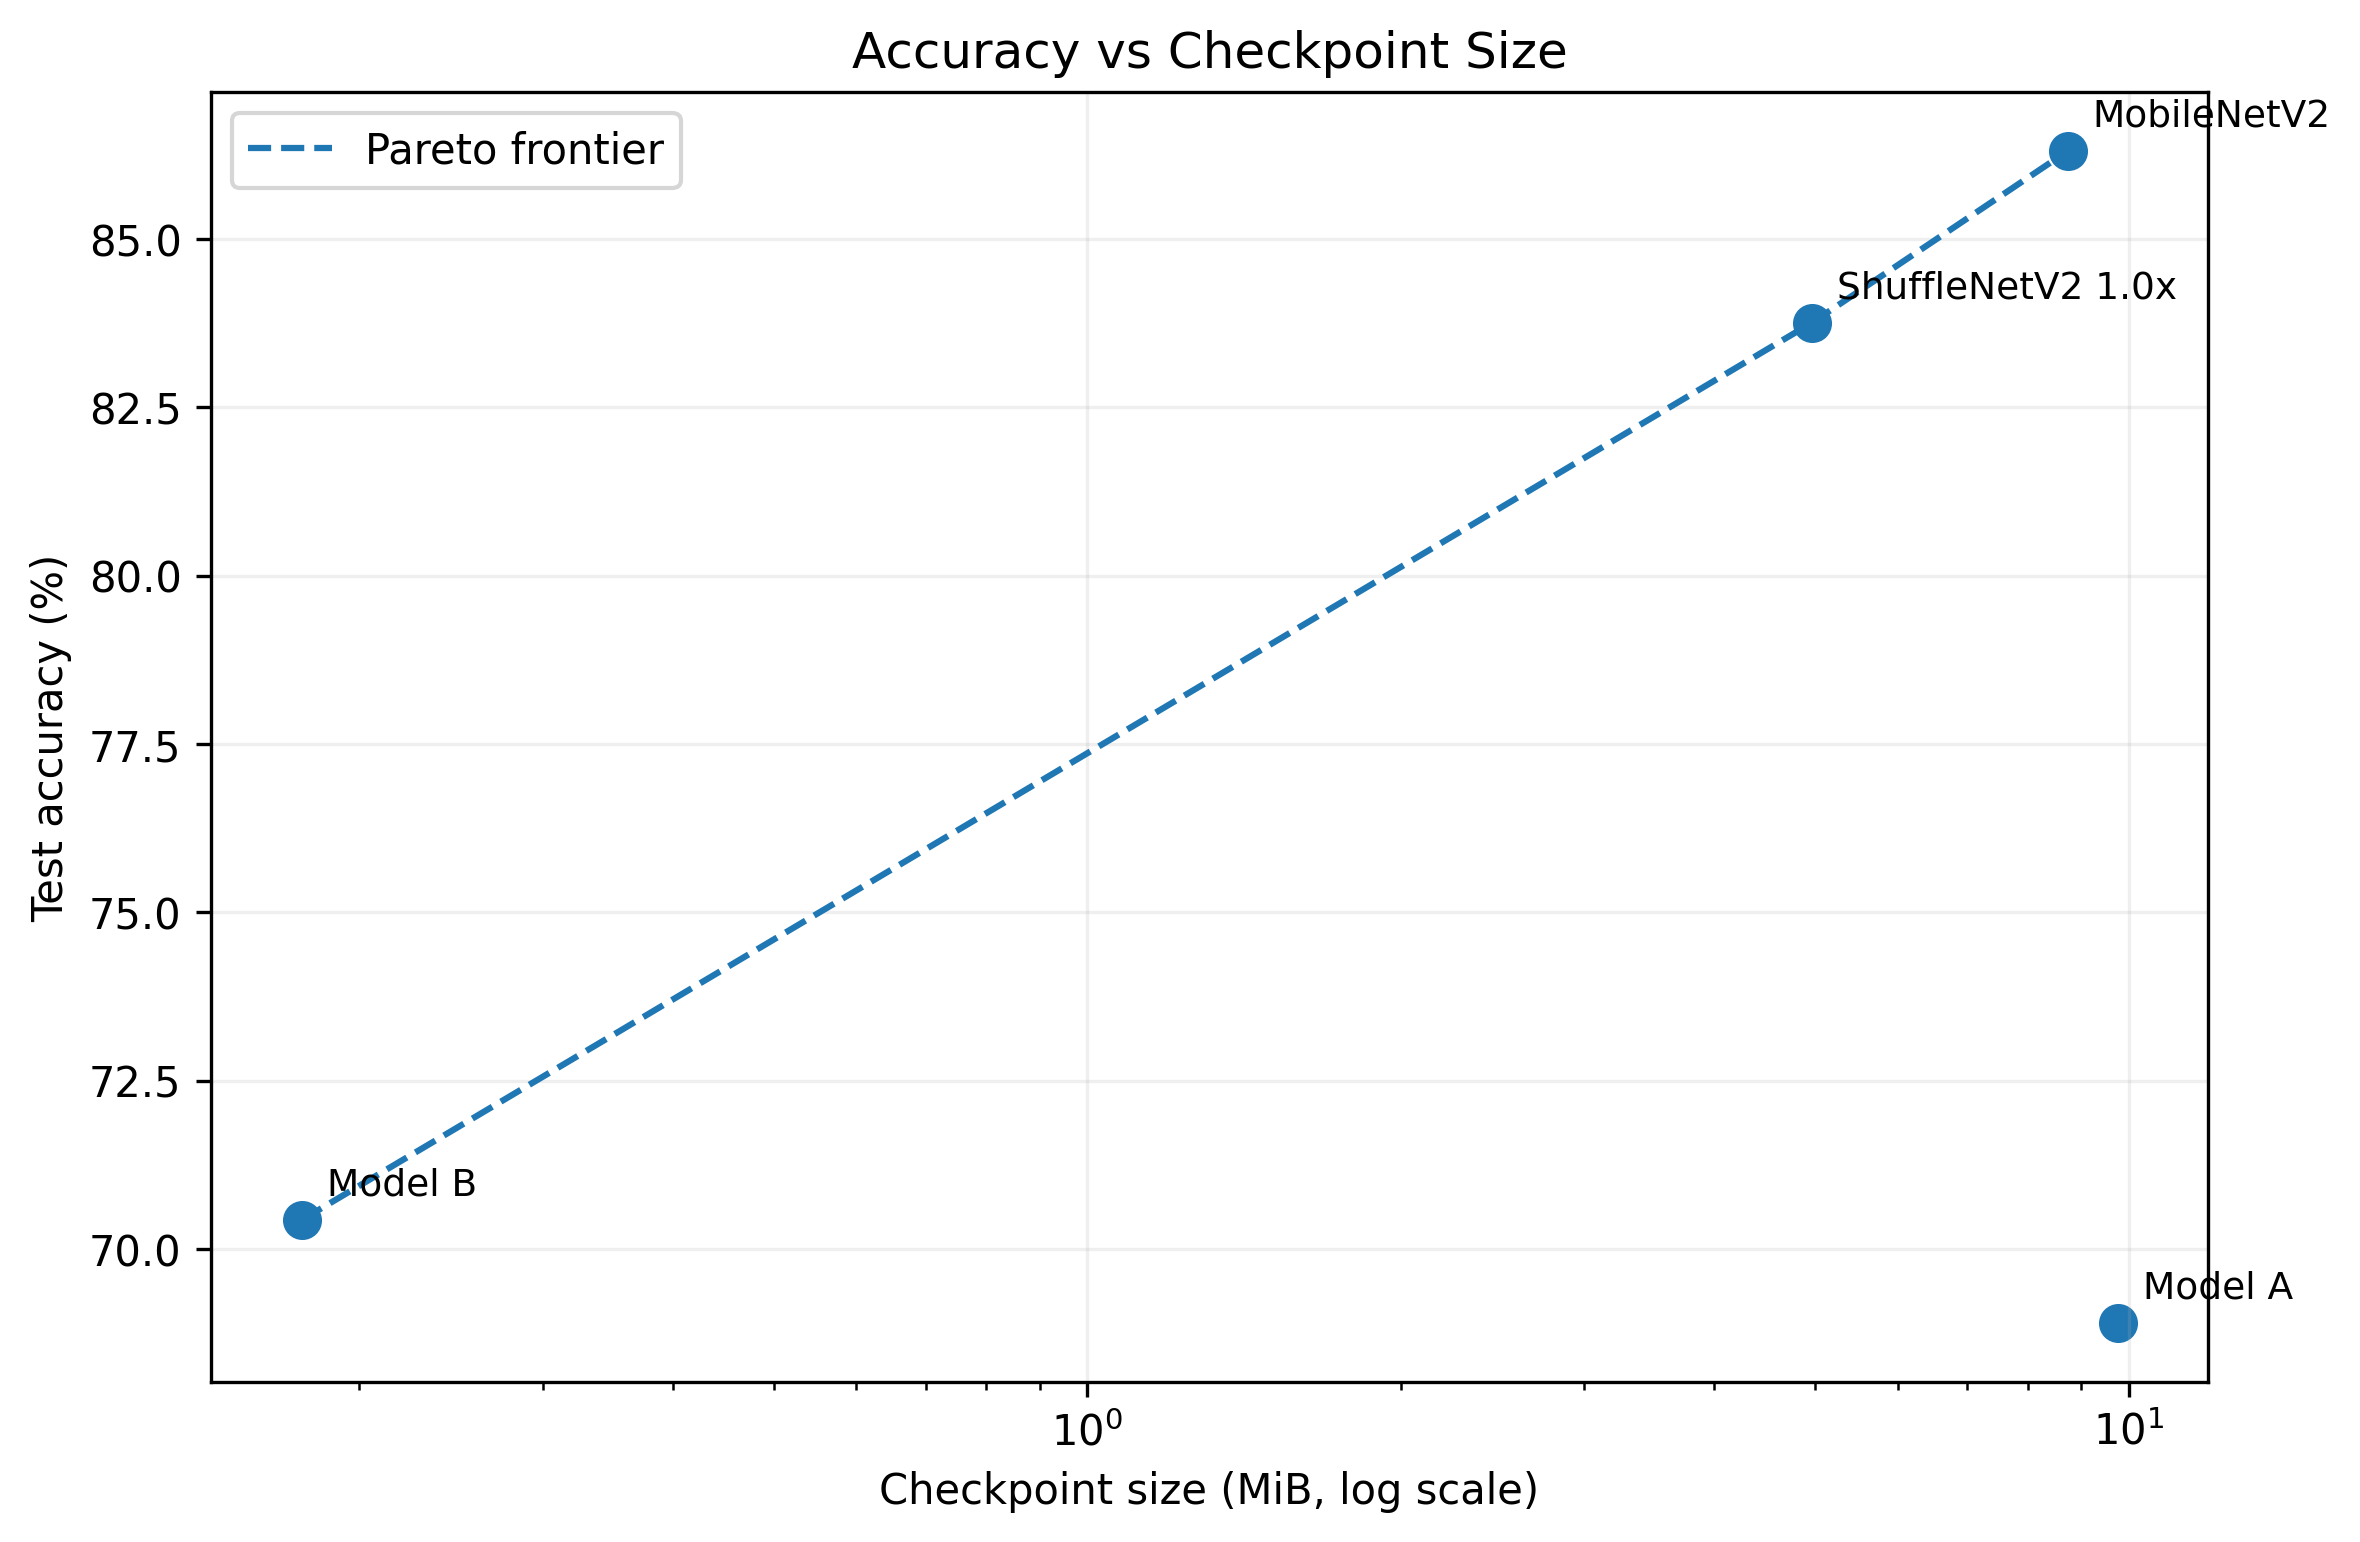
\includegraphics[width=\linewidth]{task6/accuracy_vs_model_size.png}\caption{Accuracy vs size.}\end{subfigure}\hfill
\begin{subfigure}{.49\linewidth}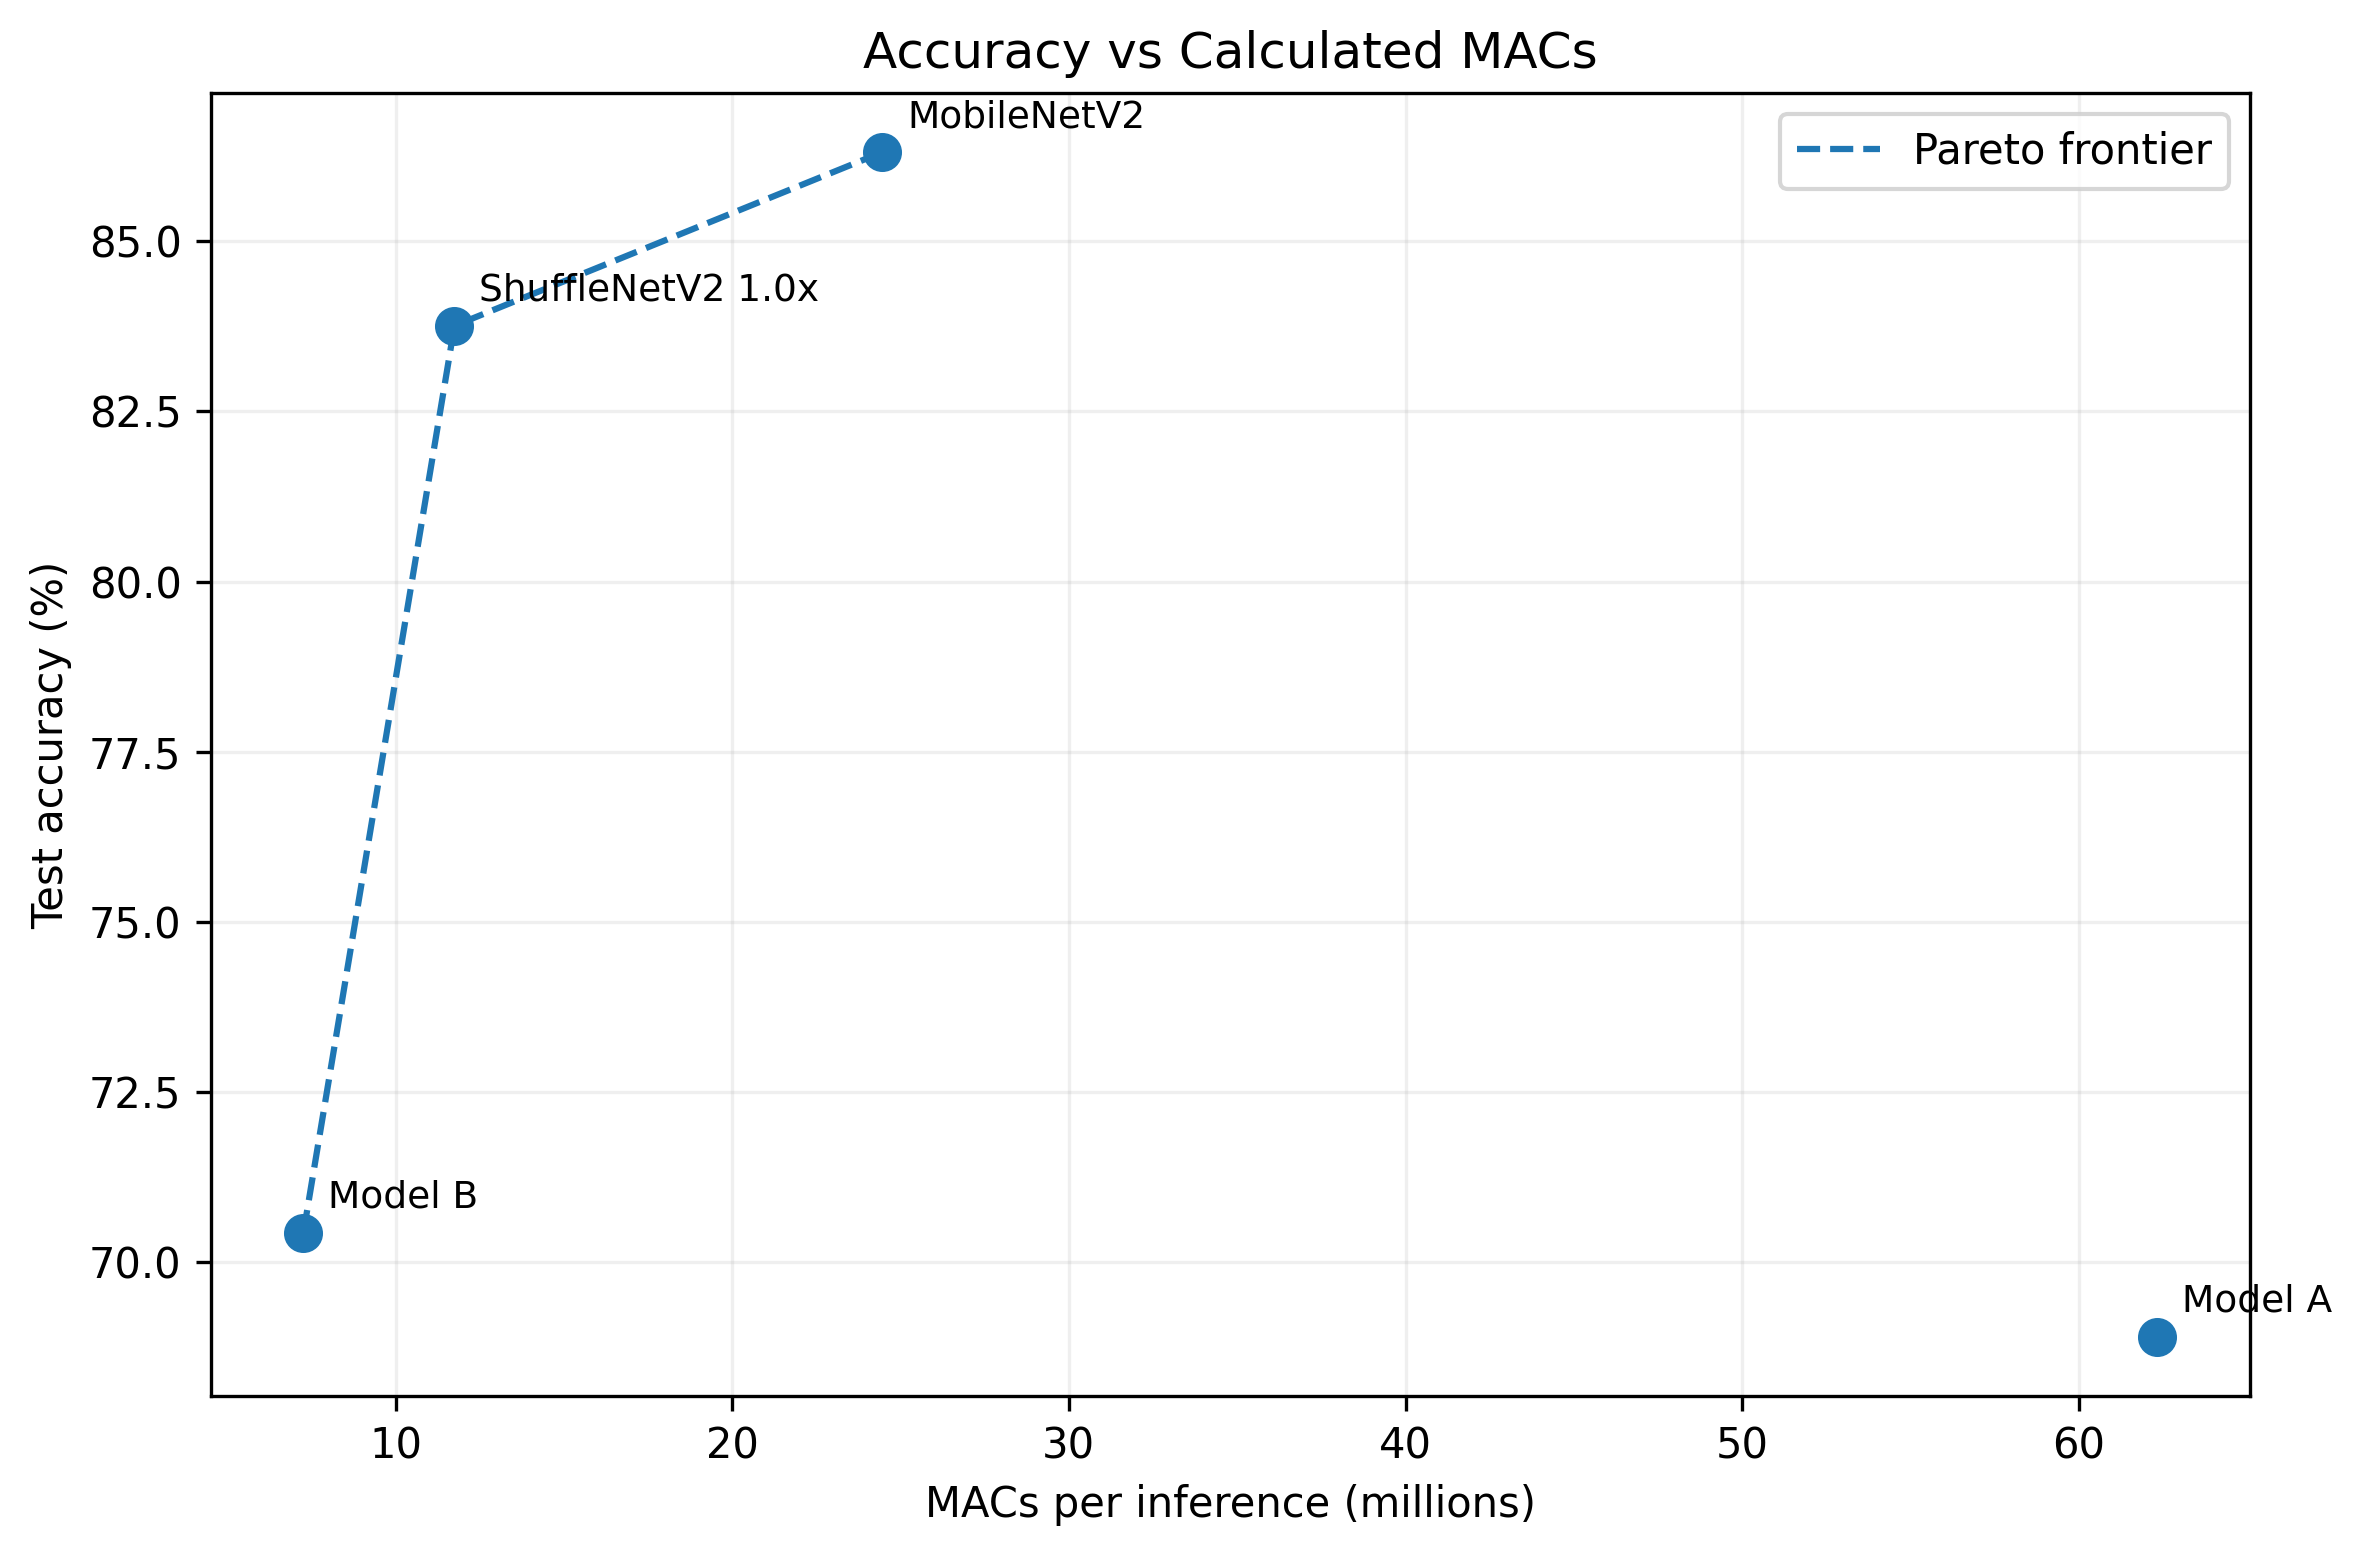
\includegraphics[width=\linewidth]{task6/accuracy_vs_macs.png}\caption{Accuracy vs MACs.}\end{subfigure}
\caption{Pareto trade-offs including Model A as a baseline.}
\end{figure}
Model A is dominated by Model B because Model B is both smaller and more accurate. Model B, ShuffleNetV2, and MobileNetV2 form distinct non-dominated operating points: minimum resource cost, balanced accuracy-efficiency, and maximum accuracy respectively.

\subsection{Advantages and Limitations}
\textbf{Model B advantages:} sub-100k parameters, very small storage footprint, lowest MAC count, simple depthwise-separable blocks, and no dependence on pre-training. Its limitations are lower classification accuracy and capacity, and difficulty on H2.

\textbf{SOTA advantages:} transfer learning provides much stronger accuracy and class-wise performance. MobileNetV2 is the accuracy leader; ShuffleNetV2 is the better efficiency compromise. Their limitations are larger memory and arithmetic requirements, and deployment still depends on peak RAM, quantization, operator support, and measured target-device latency.

\subsection{Deployment Recommendation}
\begin{itemize}
\item \textbf{Strictest resource budget: Model B.} It is the smallest model by a large margin. MCU deployment should be confirmed with quantization, peak-RAM profiling, and on-device timing.
\item \textbf{Balanced choice: ShuffleNetV2 1.0x.} It gains 13.33 percentage points over Model B while requiring substantially fewer resources than MobileNetV2.
\item \textbf{Accuracy-first choice: MobileNetV2.} It reaches 86.31\% test accuracy and 0.8805 macro F1, the best measured classification performance.
\end{itemize}

\section{Conclusion}
The experiments demonstrate a clear three-way trade-off. Model B minimizes memory and computational cost; ShuffleNetV2 provides a strong middle ground; MobileNetV2 maximizes accuracy. No single architecture is universally best, so the deployment choice should be tied to the actual memory, latency, and accuracy budget of the target edge platform.
\end{document}
